\documentclass[11pt, letterpaper]{article}
\usepackage[margin=0.8in]{geometry}
\usepackage{graphicx}
\usepackage{float}
\usepackage{hyperref}
\usepackage{amsmath}


\title{Comparative Analysis of Suffix Data Structures for Sequence Processing in Bioinformatics}
\author{Jason Hunter}
\date{\today}

\begin{document}
\maketitle



\section{Introduction}
Suffix data structures are fundamental tools in bioinformatics, particularly useful for sequence alignment, genome assembly, and sequence search tasks. 
Among the most common are suffix tries, suffix trees, and suffix arrays. 
In this analysis, I implemented and compared these three suffix data structures, examining their time and space complexities to determine the optimal choice for bioinformatics sequence processing tasks. 
During this exploration, I discovered Ukkonen's algorithm, an optimization capable of constructing suffix trees and arrays in linear time O$(n)$. 
I implemented \textit{Ukkonen's} suffix trees and arrays, comparing their performance against naive approaches, which scale quadratically O$(n^2)$ for sequences beyond 10,000 characters. 
The experiments demonstrated that suffix arrays, particularly when constructed using Ukkonen's algorithm, are significantly more efficient than suffix tries and naive suffix trees, especially for large-scale sequences. 
Suffix tries proved memory-intensive and practical only for small input sequences. 
Naive suffix trees were more efficient than tries but still consumed more memory compared to suffix arrays. 
Ultimately, the suffix array constructed using Ukkonen's algorithm emerged as the best-performing data structure, efficiently handling sequences exceeding 100,000 characters, 
and thus is clearly optimal for bioinformatics sequence processing tasks.


\section{Methods}
\subsection{Implementation}
The following data structures were implemented and evaluated:
\begin{itemize}
    \item Suffix Trie (naive approach)
    \item Suffix Tree $\&$ Suffix Array (naive approach)
    \item Ukkonen's Suffix Tree $\&$ Suffix Array (optimized approach)
\end{itemize}

\subsection{Benchmarking Framework}
Experiments were conducted to measure:
\begin{itemize}
    \item Construction time as a function of sequence size
    \item Query time as a function of both query length and sequence size
    \item Memory usage for each data structure across varying sequence sizes
\end{itemize}
Sequences used ranged from lengths of 10 to at most 10,000,000 base pairs (bp), with queries ranging from 1 to 10,000 bp. All results are displayed on log-log plots for the best visualization of the trends across these large ranges.

\section{Results}
\subsection{Construction Time Comparison}
Figure \ref{fig:construction_time} shows runtime for constructing each data structure.
\begin{figure}[H]
  \centering
  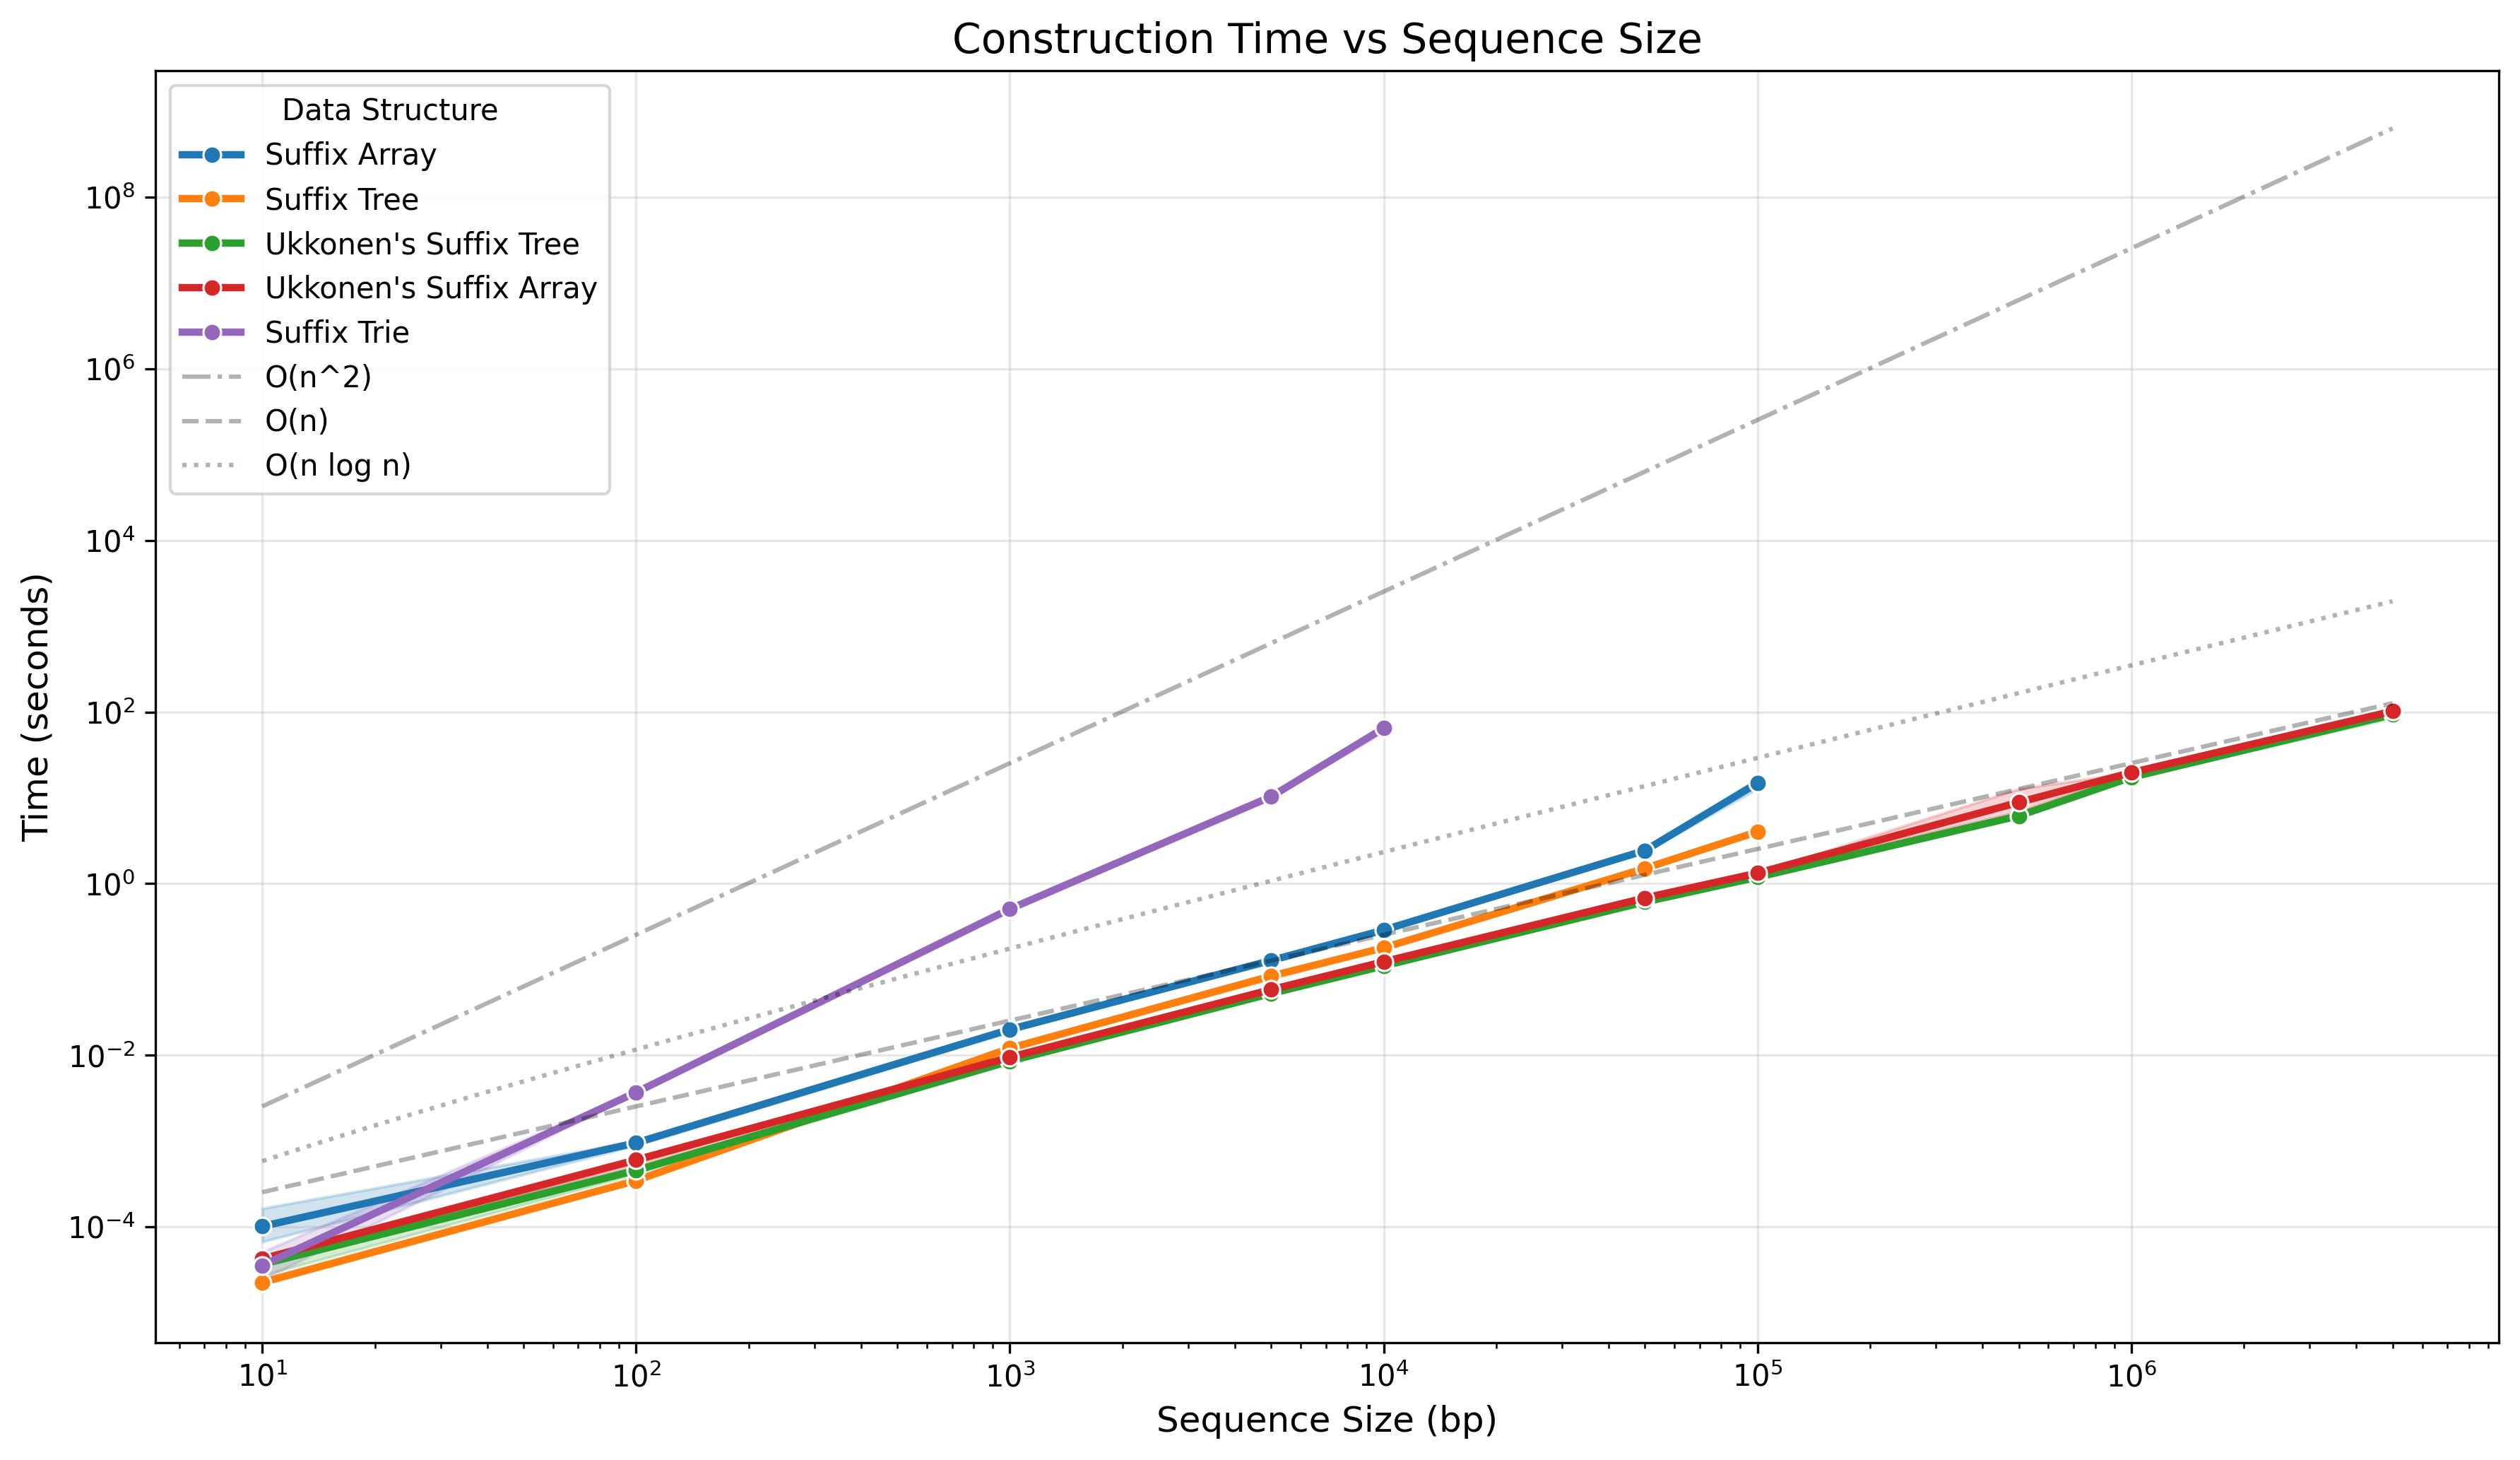
\includegraphics[width=0.7\textwidth]{../figures/construction_time.png}
  \caption{Construction time comparison for suffix tries, trees, and arrays}
  \label{fig:construction_time}
\end{figure}

Figure \ref{fig:construction_time} above displays a comparison of the runtime for constructing each of the suffix data structures, as it scales with the size of the input sequence.
The red and green lines, which represent Ukonnen's suffix tree and suffix array construction algorithms respectively, show the best scaling with the size of the input sequence.
This was the only structure that could even be run on 32gb of memory, and build trees and arrays for sequences up to 100,000,000 base pairs.
The blue and orange lines, which represent the naive suffix tree and suffix array construction algorithms respectively, show a quadratic scaling with the size of the input sequence.
At first these implementations scale well, but at around 10,000 base pairs, the runtime becomes close to quadratic, and the memory usage becomes too high to be practical.
The purple line represents the suffix trie, which is by far the slowest and most memory intensive to construct. My laptop ran out of memory when trying to construct a suffix trie for an input sequence larger than 10,000.
My gaming PC with significantly more available memory was able to run the computations at a higher level, but for practical purposes, the suffix trie is not a viable option for large input sequences.
It is clear that the suffix array constructed using Ukonnen's algorithm is the most efficient data structure in terms of construction time, and is the best choice for large input sequences,
while the suffix trie is the least efficient and should be avoided for large input sequences. \\

\newpage
\subsection{Query Time Comparison}

Figure \ref{fig:query_time} illustrates query runtime performance across suffix data structures as sequence size scales upward.

\begin{figure}[ht]
  \centering
  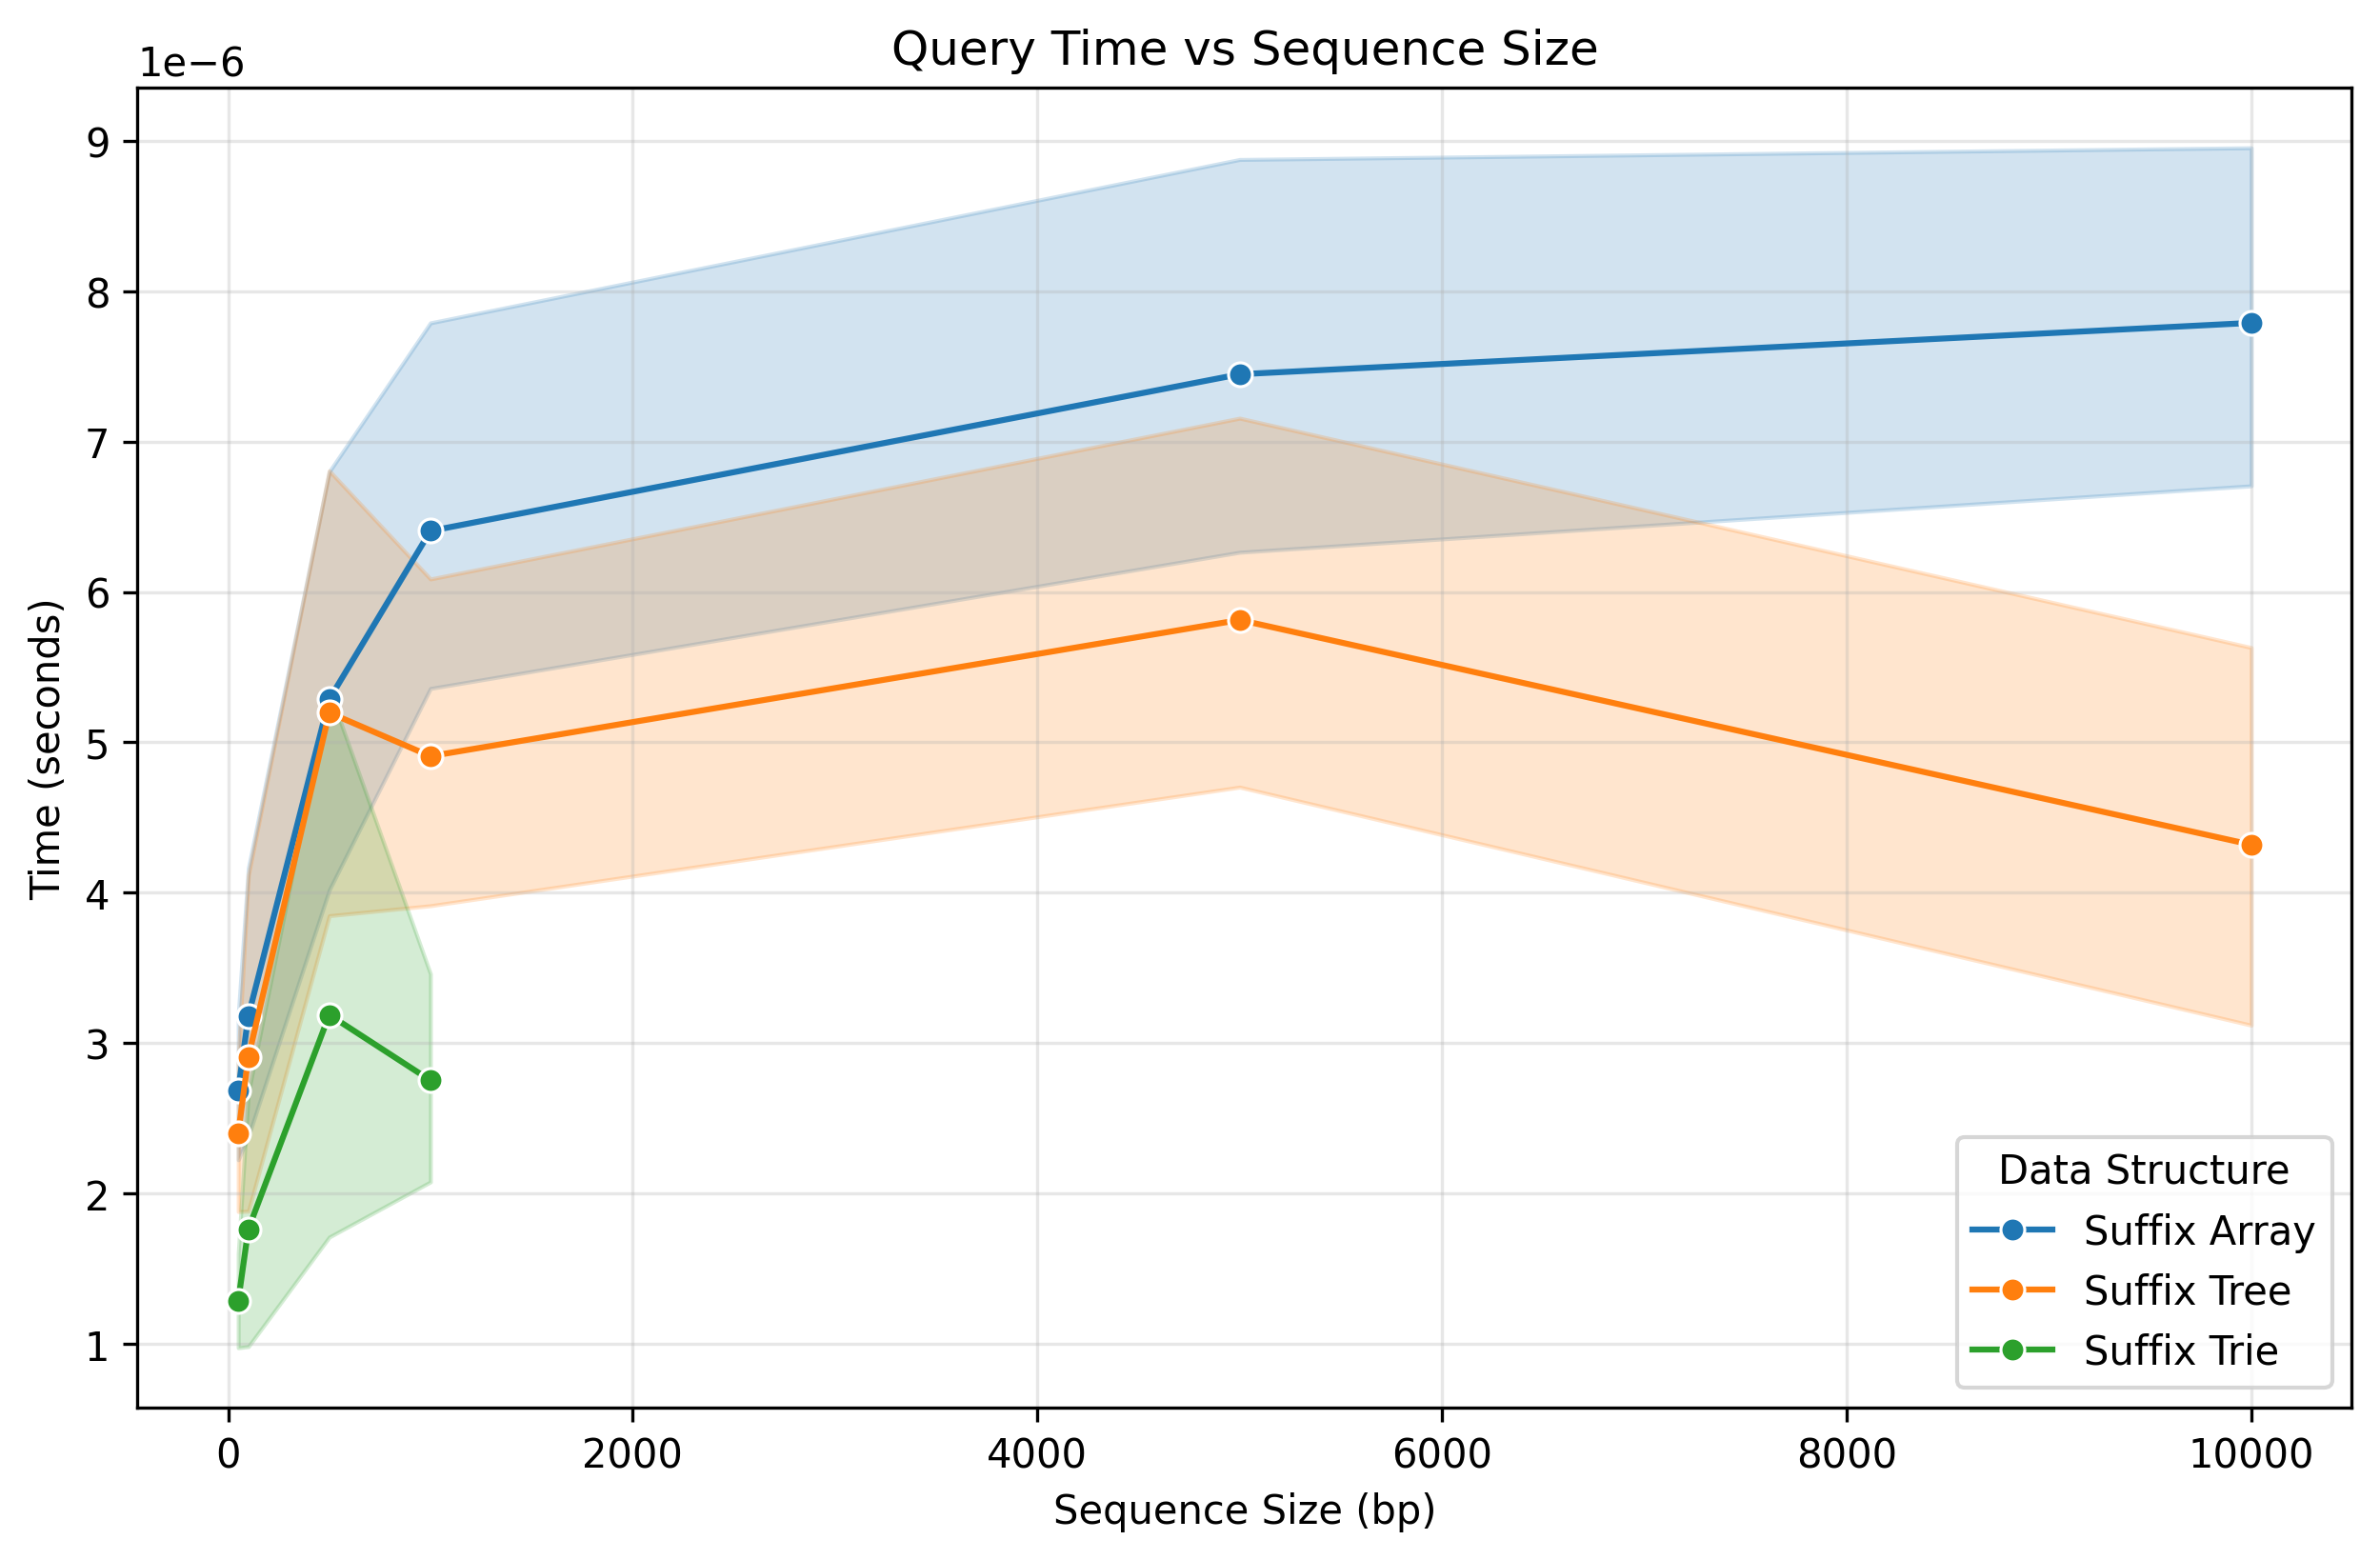
\includegraphics[width=0.7\textwidth]{../figures/query_time_by_size.png}
  \caption{Query runtime comparison for suffix tries, trees, and arrays.}
  \label{fig:query_time}
\end{figure}

Interestingly, suffix tries performed comparably or slightly better for small queries and sequences; 
however, their practicality diminishes rapidly as sequences increase in size, consistent with the trends observed previously. 
\subsection{Memory Usage Comparison}

Figure \ref{fig:memory_usage} shows memory consumption across data structures as sequence size increases.

\begin{figure}[ht]
  \centering
  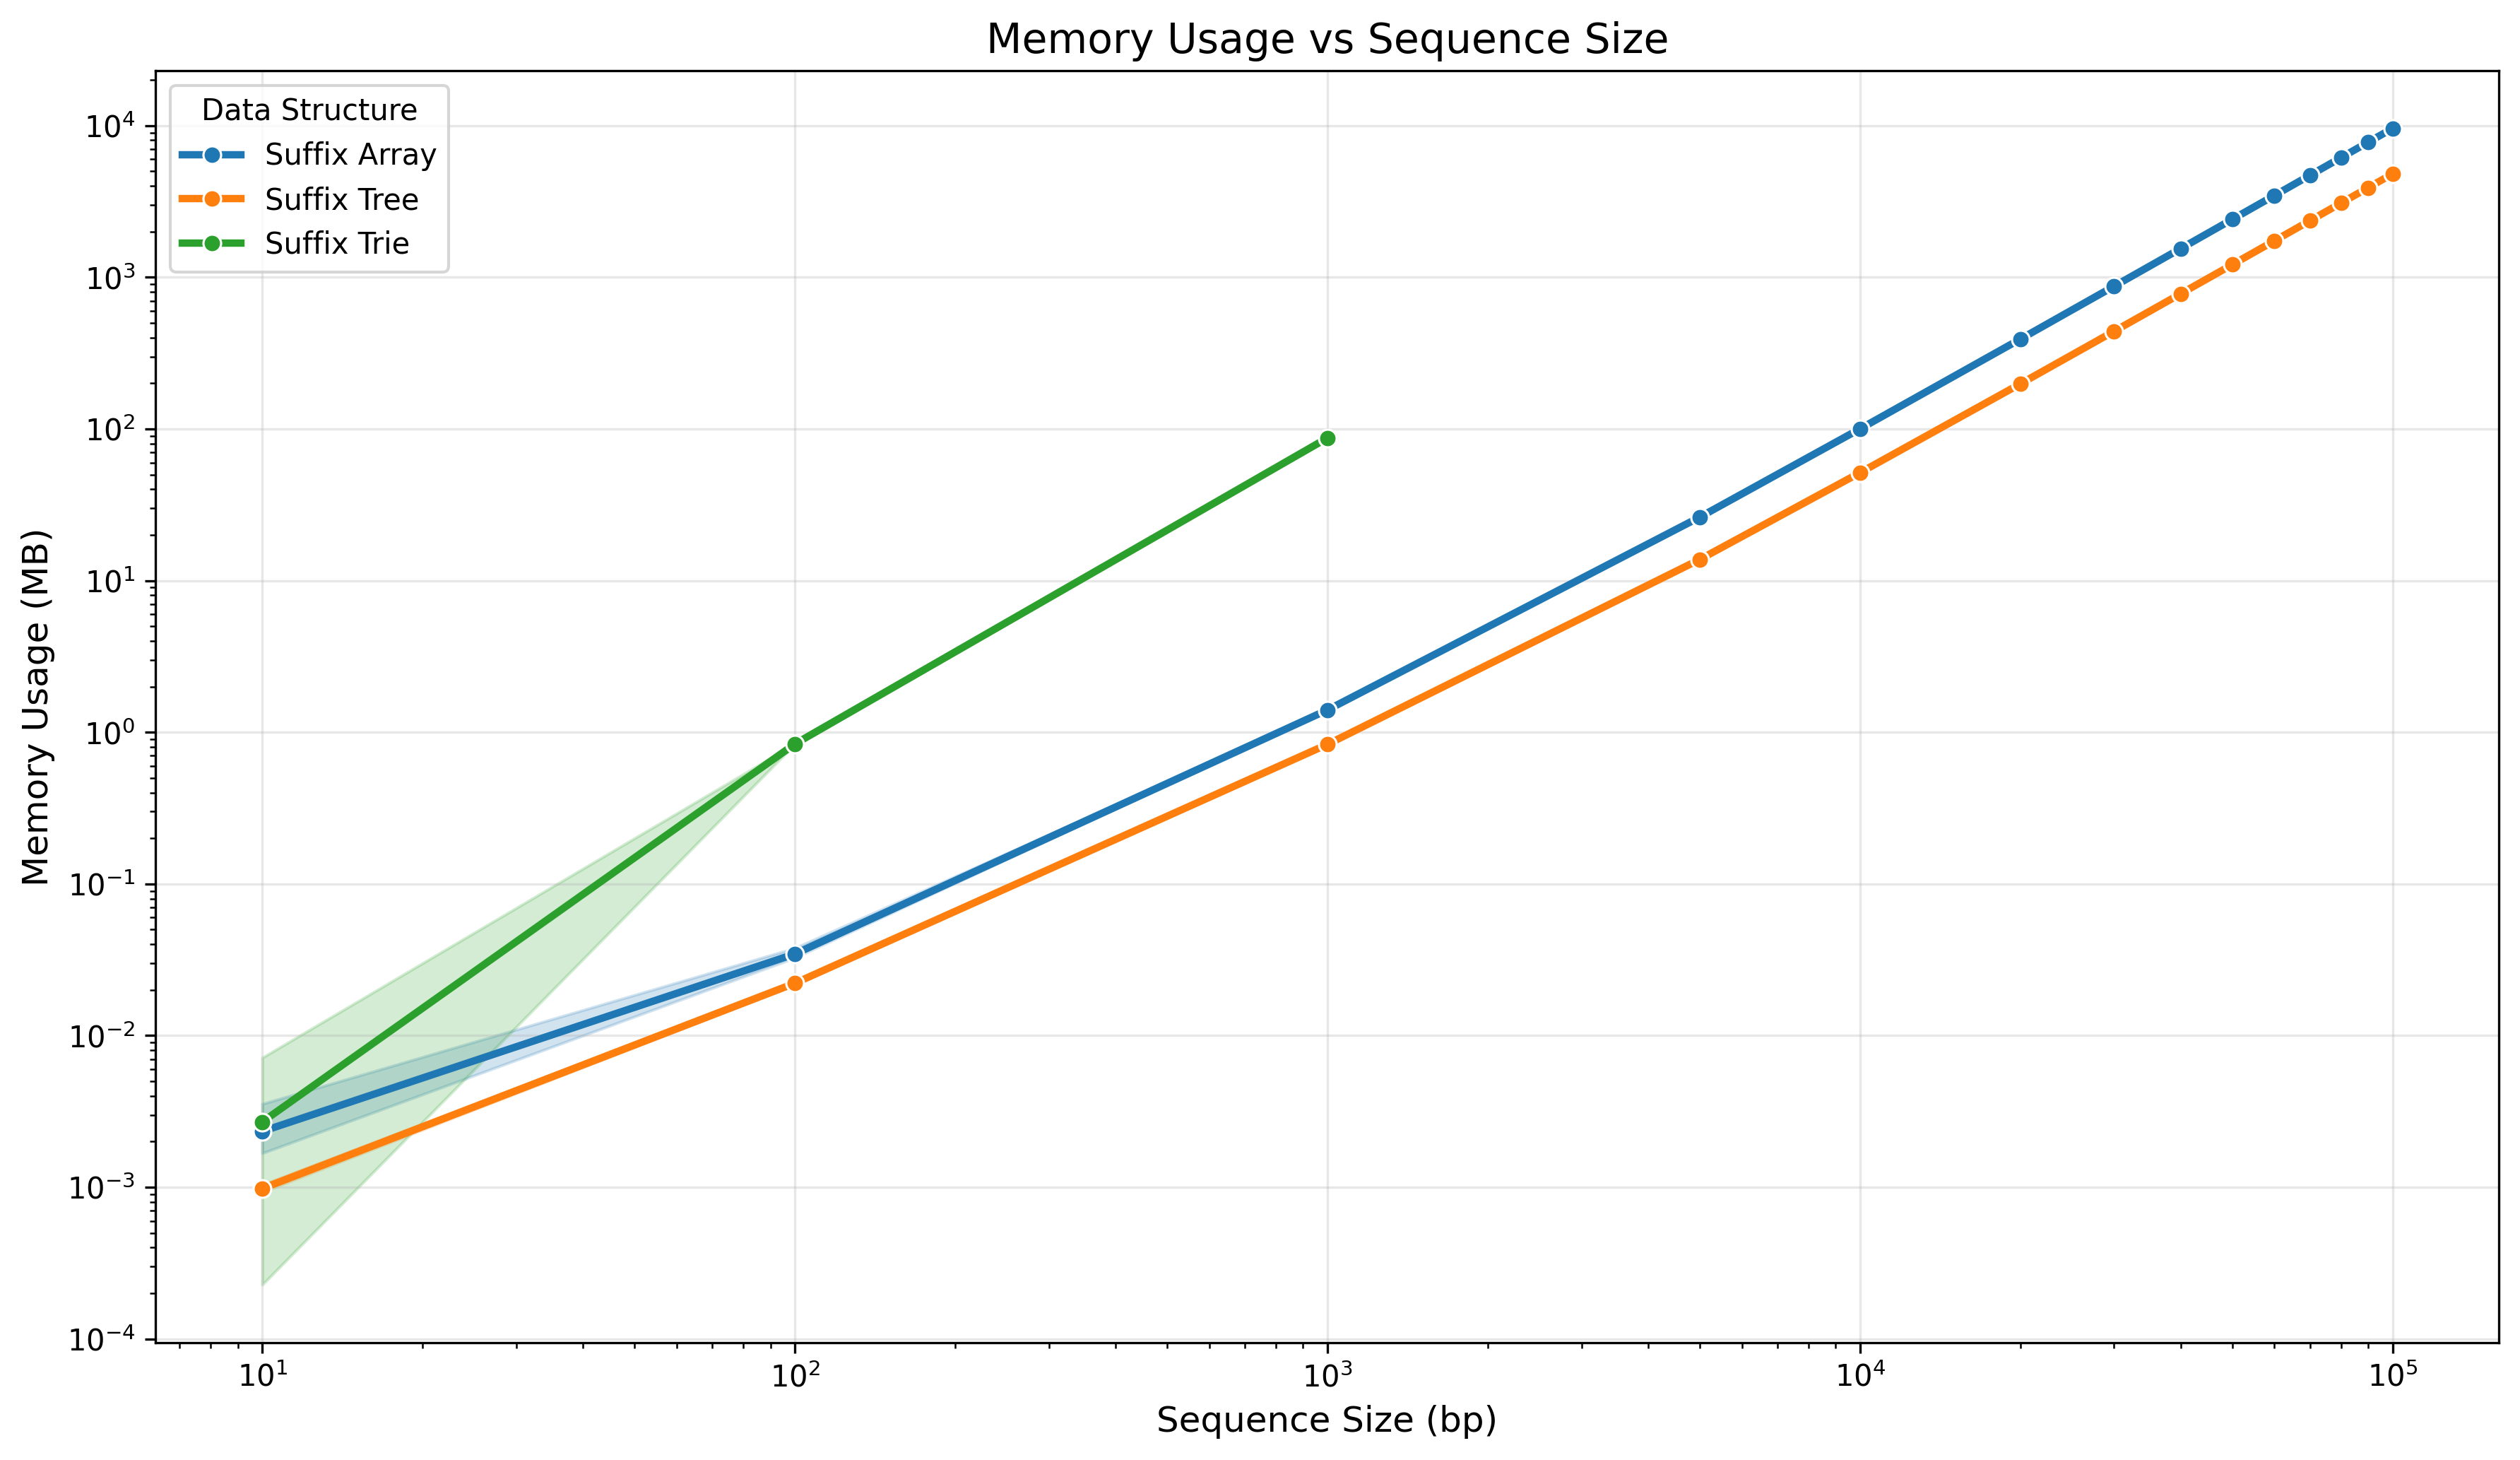
\includegraphics[width=0.7\textwidth]{../figures/memory_usage.png}
  \caption{Memory usage comparison for suffix tries, trees, and arrays.}
  \label{fig:memory_usage}
\end{figure}

Suffix tries consume significantly greater memory than other structures, 
rapidly becoming nonviable as input size grows. Conversely, Ukkonen’s suffix arrays and trees consistently display efficient, 
linear growth in memory usage. 
Naive suffix arrays and trees remain less efficient than Ukkonen’s implementation but notably more efficient than tries.

\section{Conclusion}
The analysis that I conducted ultimately revealed that the suffix array constructed via Ukkonen’s algorithm offers the best balance of construction time, query speed, and memory efficiency. 
Suffix tries, despite theoretical benefits in small-scale scenarios, proved practically infeasible due to excessive memory requirements. 
Consequently, Ukkonen's suffix array is recommended as the best suffix structure to use for large-scale sequence processing tasks.

\begin{figure}[htbp]
  \centering
  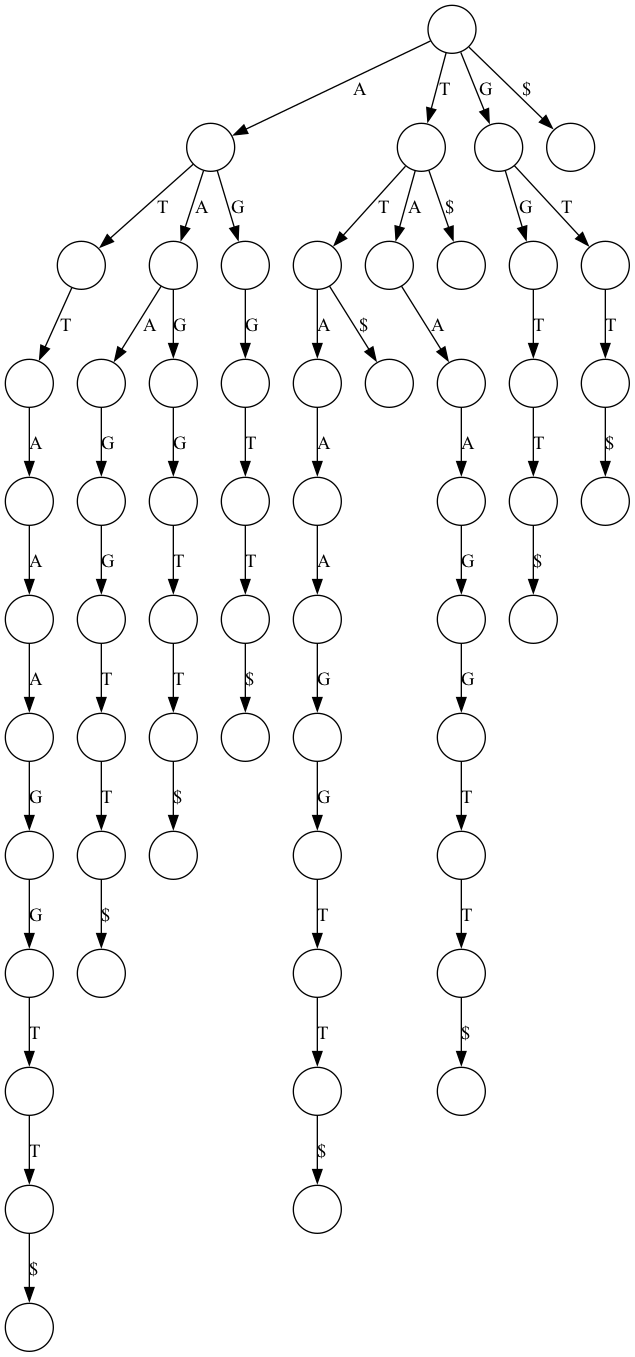
\includegraphics[scale=0.5]{../pngs/ukkonens_suffix_tree/wuhana-hu_0-10.png} % Adjust scale factor as needed
  \caption{Ukkonen's Suffix Tree for the region 0-10 of the Wuhan-Hu reference genome}
  \label{fig:ukkonens_suffix_tree}
\end{figure}

\subsection{Installing GraphicViz}
To install GraphicViz, the package used to generate the tree visualization above, run the following command:
\begin{verbatim}
$ pip3 install git+https://github.com/cjdrake/ipython-magic.git
\end{verbatim}

\newpage

\section{Reproducibility}
\subsection{Commands to collect this data and reproduce the results}
I ran these commands to generate and collect the data for the figures in this report. \\
\textbf{NOTE:} You may need to install some dependencies specified in the README.md file.
\begin{verbatim}
$ git clone https://github.com/cu-compg-spring-2025/assignment-6-suffix-index-JasonHunter95.git
$ cd assignment-6-suffix-index-JasonHunter95
$ python3 src/benchmark.py
\end{verbatim}

\subsection{Commands to run the suffix trie, tree, and array visualizations}
\textbf{NOTE:} You may need to install some dependencies specified in the README.md file and section 4 of this document. \
\begin{verbatim}
$ python3 src/suffix_trie.py \
--string BANANA \
--query ANANA NANA ANA A NA $ BANANA$
\end{verbatim}

\subsection{Commands to visualize a region of a FASTA file for the suffix structures}
\begin{verbatim}
$ python3 src/suffix_trie.py \
--reference data/chr22.fa.gz \
--query ACGT \
--region 18800-18900
\end{verbatim}

\begin{verbatim}
$ python3 src/suffix_tree.py \
--reference data/chr22.fa.gz \
--query ACGT \
--region 18800-18900
\end{verbatim}

\begin{verbatim}
$ python3 src/suffix_array.py \
--reference data/chr22.fa.gz \
--query ACGT \
--region 18800-18900
\end{verbatim}

\begin{verbatim}
$ python3 src/ukonnens_suffix_tree.py \
--reference data/chr22.fa.gz \
--query ACGT \
--region 18800-18900
\end{verbatim}

\begin{verbatim}
$ python3 src/ukonnens_suffix_array.py \
--reference data/chr22.fa.gz \
--query ACGT \
--region 18800-18900
\end{verbatim}

To reproduce: clone the repository, 
ensure that you are in the root directory and run the above commmands.
The data files are located in the data directory
and the scripts are located in the src directory
in the repository root.

\end{document}